\subsection{Evaluation metrics} \label{eval_metrics}

In this section, we present evaluation metrics that are commonly used in the literature. Choosing the right metric is very important when measuring the performance of the model. Before doing so, one should first decide which aspects of the use case are the most relevant, as different metrics measure different things. For instance, a model can be highly accurate but output few subjects. Accuracy is more relevant than completeness for some use cases, and in others, it is the other way around.

In section \ref{eval_metrics_flat}, we discuss evaluation metrics that can be used with any set of subjects, whether they have a hierarchy or not. These metrics are binary: an assignment is either right or wrong, there is nothing in between. We then look at metrics that were designed specifically for hierarchical sets of subjects, in section \ref{eval_metrics_hierarchy}. These metrics take into account how far the guessed subjects are from the correct ones, e.g. by looking at their common ancestors in the hierarchy. Such metrics are better suited for hierarchies of subjects, as accuracies can be evaluated more precisely.

Finally, we look at precision-recall curves in section \ref{eval_metrics_curve}. This metric overcomes the issue of picking a threshold value for the assignment probabilities, which is a subjective decision and strongly impacts the performance of the model. For example, for a threshold of 80 \%, we assign all subjects to documents whose probability scores are at least 80 \%. This determines how many subjects are assigned, and affects the performance of the model in the metrics presented in the previous sections.

Once we have presented all these metrics, we pick the ones we find suitable for our approach in section \ref{eval_metrics_our}. We have chosen metrics that consider the incompleteness of our evaluation set, which includes only a few subjects per document, if any.

\subsubsection{Flat metrics} \label{eval_metrics_flat}

Flat evaluation metrics are those that don't consider the hierarchy of the subjects, or any relationship between subjects, for that matter. Each assignment is considered to be either right or wrong. There are two main types of flat metrics \cite{giraldo2015evaluation}:

\begin{enumerate}
    \item \textbf{label-based metrics}, which evaluate the performance for each label (i.e. subject, in our case), and
    \item \textbf{example-based metrics}, which evaluate the performance for each example, which in our case means a document in the evaluation set.
\end{enumerate}

We will look into both families of flat metrics, as well as some of their variations, in the following sections.

\paragraph{Label-based metrics} \mbox{}

The three most common label-based metrics for text classification are precision, recall and the F-score \cite{sebastianini2002machine}. They are all computed with the number of true positives (TP), false positives (FP), true negatives (TN) and false negatives (FN). In our case, a TP is a correctly assigned subject, whereas a FP is an incorrectly assigned subject. Analogously, a TN is a subject that was correctly discarded, and a FN is a subject that is not assigned, but should have been. Thus, \textit{true} and \textit{false} define if the decision has been right or wrong, and \textit{positive} and \textit{negative} express if the subject was assigned or not.

\textit{Precision} ($P$ in the formula below) describes how often assignments are correct. \cite{sebastianini2002machine} refers to precision as the \textit{degree of soundness} of an index. A low precision means that many of the assigned subjects are wrong, whereas a high precision means that few errors were made. It is important to note that this metric does not consider the number of assignments. For example, a model can have perfect precision (i.e. $P=1$) by only assigning one subject to a document. This method is inferior to another method that assigns thousands of subjects, with a lower precision of, say, $P=0.9$. Therefore, precision is usually evaluated together with recall.

$$ P = \frac{TP}{TP + FP} $$

\textit{Recall} ($R$ in the formula below) describes how many of the made assignments are correct, in contrast with how many correct assignments are missing. \cite{sebastianini2002machine} describes recall as the \textit{degree of soundness} of an index, which makes sense looking at the example above: it is not sound, given it has only made one assignment. Even if this single assignment is correct, many other correct assignments are missing.

$$ R = \frac{TP}{TP + FN} $$

Precision and recall are often combined, as they measure two important aspects of the assignments and complement each other very well. The \textit{F-score} combines precision and recall with a parameter $\beta$, which determines the relative importance of them \cite{medelyan2008domain}. $\beta$ is usually set to one, resulting in the harmonic mean of precision and recall, shown in the formula below.

$$ F_1 = 2 \frac{P \cdot R}{P + R} $$

\paragraph{Averaging methods} \mbox{}

The three metrics presented above can be computed in three different ways:

\begin{enumerate}
    \item \textbf{Micro-average}: all results are considered at the same time.
    \item \textbf{Macro-average}: results are grouped by subject.
    \item  \textbf{Sample-based average}: results are grouped by document.
\end{enumerate}

Macro-averaged metrics consider all assignments at once regardless of the subject or the document. The metric is computed once with all assignments. We illustrate this below with the formula for the macro-averaged precision.

$$ P_{macro} = \frac{1}{|S|} \sum_{s \in S} P_s  $$

Micro-averaged metrics, on the other hand, compute the metric for each subject separately, and then average over the results. Below we show the formula for the micro-averaged precision.

$$ P_{micro} = \frac{\sum_{s \in S} TP_s}{\sum_{s \in S} TP_s + FP_s}   $$

Each of these aggregation methods has its advantages and disadvantages: which metric or aggregation method is better depends on the application \cite{toepfer2020fusion}. For instance, the $F_1$-score does not consider TN, as its value is dominated by the number of TP \cite{gargiulo2019deep}. Therefore, smaller classes have little influence in the resulting score when micro-averaging. This is not an issue for use cases where the number of correct assignments matters more than having a consistent performance across labels. On the other hand, macro-averaged results give an equal weight to each class, and is better suited for cases where all subjects are equally important, regardless how often they are assigned to documents.

\paragraph{Example-based metrics} \mbox{}

Example-based metrics, as mentioned at the beginning of this section, evaluate examples of the evaluation set instead of labels. In our case, an example is a document in the evaluation set. Studies indicate that example-based metrics are better suited for multi-label settings, as they consider all subjects simultaneously \cite{giraldo2015evaluation}. Precision, recall and F-scores can also be computed regarding the intersection of the set of predicted subjects $\hat{Y}_d$ with the set of true subjects $Y_d$ \cite{gargiulo2019deep}. For instance, the \textit{example-based precision} ($P_{EB}$ in the formula below), estimates how many predicted labels are correct.

$$ P_{EB} = \frac{1}{|D|} \sum_{d \in D} \frac{|Y_d \cap \hat{Y}_d|}{|Y_d| + |\hat{Y}_d|} $$

\paragraph{Accuracy} \mbox{}

Accuracy does not depend on the micro- or macro-average, and is an alternative to precision and recall \cite{gargiulo2019deep}. However, it is not often used in text classification because the large denominator (the number of subjects) makes this metric insensitive to variations in the number of correct decisions \cite{sebastianini2002machine}. Another issue is that, given that in multi-label settings there are usually many more true negatives than true positives, making no assignments often yields the best accuracy. This does not happen with the F1-score.

$$ Acc = \frac{\sum_{s \in S} \frac{TP_s + TN_s}{TP_s + TN_s + FP_s + FN_s}}{|S|} $$

\subsubsection{Hierarchical metrics} \label{eval_metrics_hierarchy}

Hierarchical metrics are designed specifically for hierarchical sets of subjects. They take into account how far the guessed subjects are from the correct ones, e.g. by looking at their common ancestors in the hierarchy. For example, if a document is assigned the subject \textit{k-nearest neighbors}, which is a clustering algorithm, predicting the subject \textit{neural network} is closer than \textit{urban planning}, although both predictions are wrong. Hierarchical metrics aim to recognize the difference between both predictions, penalizing \textit{urban planning} more than \textit{neural network}.

These metrics assume that the assignments are consistent. If a subject is assigned to a document, all its ancestors in the hierarchy should also be assigned to the same document. In the case of \textit{k-nearest neighbors}, its parents would be \textit{clustering algorithms}, \textit{machine learning} and \textit{computer science}, for example. Precision, recall and F-scores can be adapted to hierarchical structures of subjects by considering the sets of predicted and true labels \cite{gargiulo2019deep}. In fact, they already do so in their example-based formulations, if the assignments are consistent with the hierarchy.

Common ancestors between predicted and true subjects increase the performance of the model in these metrics, as they are all included in the sets of subjects. However, adding all the ancestors can also lead to overestimating errors when the hierarchy has many levels. If assigned subjects have many ancestors, the sets of assigned and predicted subjects will be very large and may differ greatly, even if the predicted and assigned subjects are not so semantically different.

\cite{kosmopoulos2015evaluation} proposes several metrics that, instead of comparing complete sets of subjects, looks for the common ancestors of true and predicted subjects. The \acrfull{lca} of two nodes is the node that is furthest from the root, considering the common ancestors of the two nodes. As we don't know how to map the predicted subjects to the true ones, we consider all true subjects when looking for the \acrshort{lca} of a predicted subject. Thus, each predicted subject is compared to its most similar subject in the true set of subjects. The same is done the other way around, i.e. looking for the \acrshort{lca} for each true subject with the set of predicted subjects. Then we have again two sets of subjects, and the common metrics such as precision, recall and F-scores can be computed.

\subsubsection{Precision-recall curves} \label{eval_metrics_curve}

\acrfull{mlc} models usually output assignment probabilities for the subject, finally assigning those that are above a certain threshold. The choice of a threshold depends on what the assigned subjects are going to be used for. For instance, if one wants to relate documents to one another, a lower threshold will be picked, so that each document has more subjects, which results in more connections to other documents. On the other hand, if wrong predictions are not acceptable, like for example in the biomedical field, a higher threshold would be better.

Therefore, research on \acrshort{mlc} is usually evaluated with precision-recall curves \cite{wehrmann2018hierarchical}, which plot the trade-off between precision and recall for different threshold values (i.e. from zero to one). To enable the comparison between different curves, the area under the curve is measured. which results in a scalar that can be easily compared across methods. A higher area under the curve means that both the recall and the precision are high. Therefore, models with higher areas are considered better.

\subsubsection{Our metrics} \label{eval_metrics_our}

The researchers that use the metrics presented above use complete evaluation sets, where the subjects have been manually assigned to the documents. They are also noisy, given the lack of inter-indexer consistency \cite{csomai2007investigations}, but each document has multiple assigned subjects, which together describe their ``aboutness''. Our evaluation sets, as discussed in section \ref{eval_datasets_summary}, are sparse. They include only a few assignments per document, usually just one and sometimes none. We have to take this aspect into account when picking evaluation metrics.

Here we present the two metrics we use to evaluate the two approaches. The first one, called accuracy, checks if the correct subject is included among the top $n$ subjects output by a given model. The second metric, called \acrfull{lcas}, quantifies the \acrfull{lca} between the correct subject and the top $n$ subjects output by a model. The second metric is only used in the handwritten evaluation set, as the other two evaluation sets only consider fields, which don't have any ancestors.

\paragraph{Hit rate} \mbox{}

\textit{Hit rate} is an intuitive metric that measures how often the correct subject is within the top $n$ candidates output by a model as a percentage. We consider each assignment individually, checking if it is in the list of candidates or not. Then we divide the number of correct inclusions by the number of total checks. If a document has multiple assignments, each are considered independently.

For the \acrshort{ddc} and venue evaluation sets, where there are only 19 possible assignments, the number of candidates ranges from one to five. For the handwritten evaluation set, where there are 2,157 possible assignments, we consider 5, 10, 20, 30 and 50 candidates. Recall that the subject assignments of this dataset are not necessarily those that best represent their respective documents, and therefore are not expected to be on their top 5 or 10 candidates.
 
This metric is analogous to the one used in object recognition tasks in ImageNet \cite{russakovsky2015imagenet}, called \textit{error rate}, where they count misses instead of hits. Considering a variable number of candidates, they measure how often the correct assignments are not included. Thus, a lower error rate is better. In our case, where we count hits, a higher hit rate is better.

\paragraph{LCAS} \mbox{}

The \acrfull{lcas} is based on the evaluation metric proposed in \cite{kosmopoulos2015evaluation}, which quantifies the similarity of two subjects based on their \acrfull{lca}. \cite{kosmopoulos2015evaluation} concludes that a set-based version of the F1-score is the best metric for most use cases, but that pair-based metrics might be better for special cases. As stated above, our evaluation set is special because of its incompleteness. It contains one assignment per document, if any. Therefore, we adapt their metric to our case.

We define this metric by considering a \textit{correct subject}, which is the subject assigned to a document in the evaluation set, and a \textit{candidate subject}, which is the subject assigned to a document by a model. The candidate subject doesn't have to be correct, i.e. it is not always the same as the correct subject. As mentioned above, the \acrshort{lca} of two subjects is the subject that is furthest from the root, considering the common ancestors of the two subjects. We quantify the \acrshort{lca} by measuring the length of the path from the root (i.e. the fields) to the \acrshort{lca}.

Given that the depths of the paths from the fields to the subjects vary depending on the subject, we divide the length of the path to the \acrshort{lca} by the length of the path to the subject. This normalizes the \acrshort{lcas}, so larger paths are not overestimated. We also add one to all paths, which is the same as adding another node above the fields. We do this, so fields don't receive an \acrshort{lcas} of zero, as their actual path length is zero. Furthermore, adding one to all paths avoids divisions by zero if the correct subject is a field.

As correct and candidate subjects may have multiple common ancestors in the same hierarchy level, we always pick the ancestor for which the \acrshort{lcas} is highest. This evaluation metric, as the first one, is parameterized by the number of candidates. The formal definition of the \acrshort{lcas} can be seen below, where $Y$ is the correct subject, $X$ is the candidate subject and $LCA(X,Y)$ is their \acrshort{lca}. $P(S)$ is the path from the root to the subject $S$, and $|P(S)|$ denotes the length of that path.

$$ LCAS(X, Y) = \frac{|P(LCA(X, Y))|+1}{|P(Y)|+1}$$

\paragraph{Example of the LCAS} \mbox{}

\begin{figure}
    \centering
    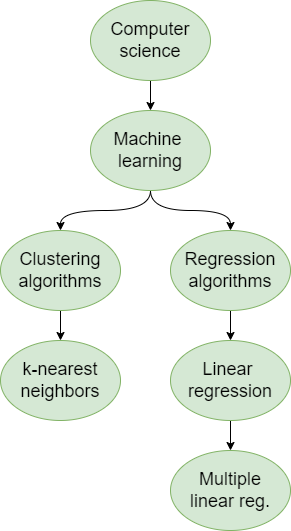
\includegraphics[width=.4\textwidth]{figures/evaluation/subject_hierarchy_example.png}
    \caption{Example of a subject hierarchy}
    \label{fig:subject_hierarchy_example}
\end{figure}

We illustrate the \acrshort{lcas} using the subject hierarchy shown in figure \ref{fig:subject_hierarchy_example}, which comprises subjects of the field \textit{Computer science}, with five hierarchy levels.

For correct subject \textit{Linear regression} and candidate subject \textit{Clustering algorithms}, the \acrshort{lca} would be \textit{Machine learning}. The path from the field \textit{Computer science} to the subject \textit{Linear regression} has length 3, as it passes through \textit{Machine learning} and \textit{Regression algorithms}. The length of the path to the \acrshort{lca} is 1. Thus, the \acrshort{lcas} for subject \textit{Linear regression} and candidate \textit{Clustering algorithms} is $\frac{1}{2}$. We show it in mathematical notation below, with each subject abbreviated to its initials for clarity.

$$ LCAS(CA, LR) = \frac{|P(LCA(CA, LR))|+1}{|P(LR)|+1} = \frac{|P(ML)|+1}{|P(LR)|+1} = \frac{2}{5} = \frac{1}{2} $$

If the correct subject were \textit{Multiple linear regression}, which descends from \textit{Linear regression}, the \acrshort{lcas} would be lower ($\frac{2}{5}$ instead of $\frac{1}{2}$). This is expected, as the descendant is further away from the \acrshort{lca}. On the other hand, if it were \textit{Machine learning}, which is an ancestor of the candidate, the \acrshort{lcas} would be $1$, which is its maximum value. This is also expected as the \acrshort{lca} is \textit{Machine learning} itself. The same \acrshort{lcas} would be achieved if the correct subject were \textit{Computer science}.

\begin{table}[]
    \centering
    \begin{tabular}{|c|c|}
        \hline
        \textbf{Correct subject} & \textbf{LCAS} \\ \hline\hline
        Computer science & 1 \\ \hline
        Machine learning & 1 \\ \hline
        Clustering algorithms & 1 \\ \hline
        k-nearest neighbors & 0.75 \\ \hline
        Regression algorithms & 0.67 \\ \hline
        Linear regression & 0.5 \\ \hline
        Multiple linear reg. & 0.4 \\ \hline
    \end{tabular}
    \caption{LCAS for several subjects where the candidate is \textit{Clustering algorithms}.}
    \label{tab:lcas_example}
\end{table}

In table \ref{tab:lcas_example}, we show several \acrshort{lcas} where \textit{Clustering algorithms} is the candidate subject. Here we can see that the \acrshort{lcas} decreases as we go deeper into the other subtree, and also that it is equal to one, the maximum value, when the correct subject is above the candidate subject in the hierarchy. Another interesting characteristic of the \acrshort{lcas} is that guesses that are further down in the hierarchy are rewarded. Thus, although the relative position of the subjects is the same, being close to a correct subject that is deeper in the hierarchy outputs a higher \acrshort{lcas}. For example, the \acrshort{lcas} of correct subject \textit{Linear regression} and candidate \textit{Regression algorithms} is $0.75$, whereas for correct subject \textit{Multiple linear regression} and candidate \textit{Linear regression}, the \acrshort{lcas} is $0.8$.
